% =========================================================
\subsection{App4-Creation of 2D Model}\label{sec:App4-Creation of 2D Model}
% =========================================================

\begin{enumerate}
%%\vspace{0.2cm}
	
\item \textbf{About 2D/3D model drawings and G-Code files}

In summary, we say that a 2D or 3D model drawing file is about providing information on what we want to produce, meaning. the visual look of the model, whereas a G-Code command file for the 2D or 3D model drawing is about providing information on specific machine instructions on how to produce, meaning, the required machining steps to produce the model.
% \vspace{0.3cm}

Similarly, we say that CAD applications generate 2D or 3D model drawings as outputs while CAM applications generate G-Code file outputs from the 2D or 3D model drawings as inputs.

The inputs to the CAD application are essentially, virtual and non-tangible ideas formed inside the human mind, that the designer wants to translate into models and drawings in software terms. 
% \vspace{0.2cm}

\item \textbf{Creation of a drawing 2D or 3D model}

Many software applications can create 2D or 3D model drawings as described at the list of  \href{https://www.pannam.com/blog/best-3d-cad-modeling-software/}{best 3D CAD modeling software}. 

Some examples of commercial and high end applications are [\href{http://www.autodesk.com/products/autocad/overview}{AutoCAD}],
[\href{http://www.solidworks.com/sw/products/3d-cad/packages.htm}{Solid Works}],
[\href{http://www.autodesk.com/products/fusion-360/overview}{Fusion 360}] and
[\href{https://www.bricsys.com/en\_INTL/bricscad/D}{BrisCAD}]. Some examples of cost-free and open source applications are [\href{https://inkscape.org/}{Inkscape}],
[\href{http://www.openscad.org/}{OpenSCAD}], 
[\href{https://www.freecadweb.org/}{FreeCAD}],
[\href{https://brlcad.org/}{BRL-CAD}] and 
[\href{https://www.blender.org/}{Blender}].


The 2D or 3D model files are normally represented as standardized \href{https://vectormagic.com/support/file_formats}{graphic vector files}. A graphic vector file is a software file that represents its graphical elements in terms of text, and this text is editable manually with a text editor application. Some examples of graphic vector files are SVG, STL, PDF (Tikz), DXF, EPS, AI, and so on. 

On the other hand, graphical images that are saved as non-graphic files (scalar bitmap) are not represented in text and so cannot be edited using a text editor. Some examples of graphic bitmap files are BMP, JPEG/JPG, PNG, GIF, TIFF/TIF and so on. Non graphic files can only be edited using special GUI applications for example, Inkscape, Adobe Illustrator, Graphic Image Manipulation Program (GIMP), PaintBrush, OpenSCAD, Blender and so on.  

\item \textbf{Example of a 2D model drawing using Inkscape}

As an example in our CNC research work, a \textbf{2D KSG drawing} was created using the open source Inkscape graphic software application. This drawing was saved in SVG/XML textual vector format. 

A visual display image of the 2D KSG drawing is provided in the next figure at the link [\ref{fig:App4-Inkscape-Display-of-2D-KSG.jpg}]. A textual(SVG/XML) listing display of the same 2D KSG drawing is provided in the next figure at the link \ref{sec:Display-KSG-SVG-XML}.

This 2D KSG drawing was selected for illustration purposes because the drawing requires both linear (straight line) and circular arc (curve) movements. The character K is made up of totally linear movements, while the characters S and G require both linear and curve movements.

\end{enumerate}

% =======================================================
\pagebreak
\textbf{Example of a 2D model KSG drawing using Inkscape}

\begin{figure}[htbp]
	\begin{center}
		\frame{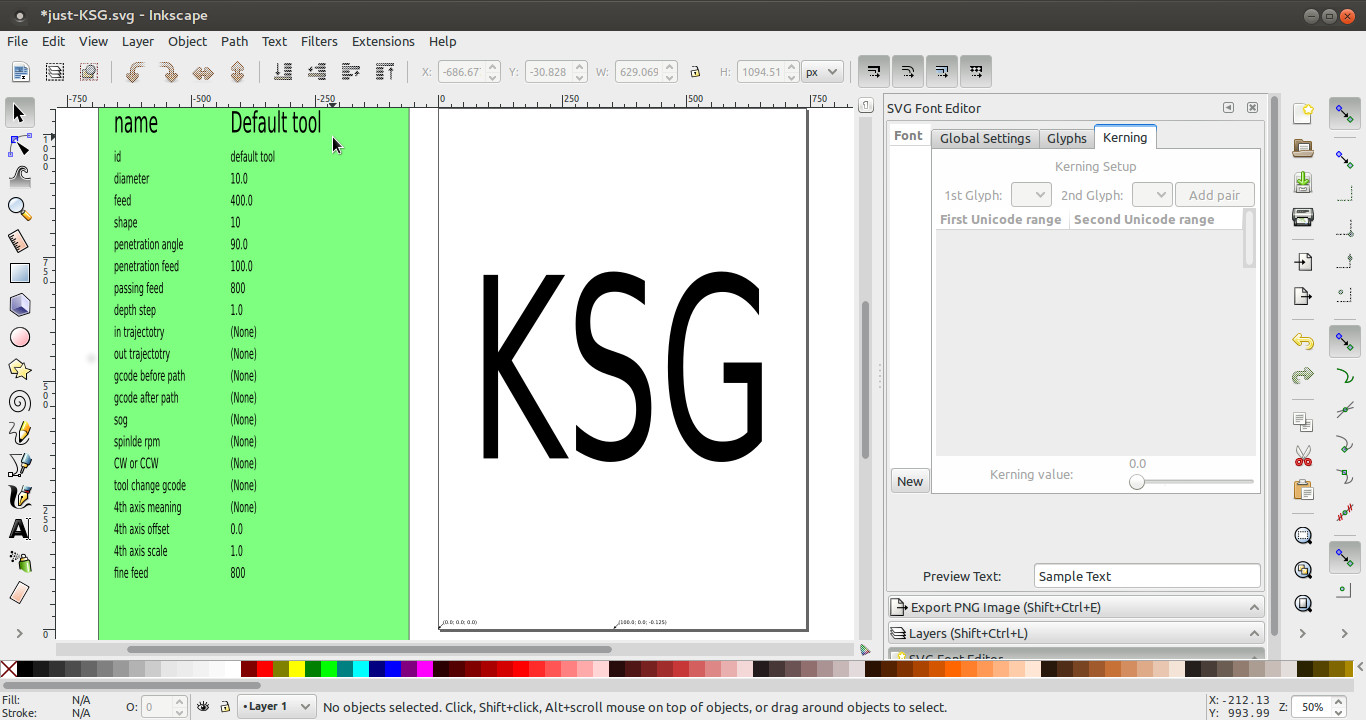
\includegraphics[width=1.3\textwidth]{./07-images/img-Ch4App/Inkscape-Display-of-2D-KSG.jpg}}
		\caption{App4-Inkscape display of 2D KSG jpg file.}
		\label{fig:App4-Inkscape-Display-of-2D-KSG.jpg}
	\end{center}
\end{figure}

% ========================================================
\pagebreak
\textbf{Display Text for 2D KSG model SVG/XML (Clipped text from 671 lines total)}

% ==========================================================
\lstset{basicstyle=\footnotesize, numberstyle=\tiny\color{blue}, frame=single, numbers=left, firstnumber=1, stepnumber=1, numbersep=1pt, xleftmargin=2.0em, framexleftmargin=1.5em, xrightmargin=0.0em, breaklines=true, breakatwhitespace=false, breakindent=5pt, prebreak=\space, postbreak=\space }
% ==========================================================

\begin{lstlisting}[caption={App4-Display Text for 2D KSG model SVG/XML}, label=App4-Display Text for 2D KSG model SVG/XML]
<?xml version="1.0" encoding="UTF-8" standalone="no"?>
<!-- Created with Inkscape (http://www.inkscape.org/) -->

<svg
xmlns:dc="http://purl.org/dc/elements/1.1/"
xmlns:cc="http://creativecommons.org/ns#"
xmlns:rdf="http://www.w3.org/1999/02/22-rdf-syntax-ns#"
xmlns:svg="http://www.w3.org/2000/svg"
xmlns="http://www.w3.org/2000/svg"
xmlns:sodipodi="http://sodipodi.sourceforge.net/DTD/sodipodi-0.dtd"
xmlns:inkscape="http://www.inkscape.org/namespaces/inkscape"
	width="210mm"
	height="297mm"
	viewBox="0 0 744.09448819 1052.3622047"
	id="svg4749"
	version="1.1"
	inkscape:version="0.91 r13725"
	sodipodi:docname="just-KSG.svg">
	<sodipodi:namedview
	id="base"
	pagecolor="#ffffff"
	bordercolor="#666666"
	borderopacity="1.0"
	inkscape:pageopacity="0.0"
	inkscape:pageshadow="2"
	inkscape:zoom="0.35"
	inkscape:cx="375"
	inkscape:cy="520"
	inkscape:document-units="px"
	inkscape:current-layer="layer1"
	showgrid="false"
	inkscape:window-width="1366"
	inkscape:window-height="689"
	inkscape:window-x="0"
	inkscape:window-y="24"
	inkscape:window-maximized="1" />
	<defs
	id="defs4751" />
	<metadata
	id="metadata4754">
	<rdf:RDF>
	<cc:Work
	rdf:about="">
	<dc:format>image/svg+xml</dc:format>
	<dc:type
	rdf:resource="http://purl.org/dc/dcmitype/StillImage" />
	<dc:title></dc:title>
	</cc:Work>
	</rdf:RDF>
	</metadata>
	<g
	id="layer1"
	inkscape:groupmode="layer"
	inkscape:label="Layer 1">
	<text
	transform="scale(0.76565133,1.3060775)"
	sodipodi:linespacing="125%"
	id="text4757"
	y="554.98346"
	x="81.874046"
	style="font-style:normal;font-weight:normal;font-size:389.44628906px;line-height:125%;font-family:sans-serif;letter-spacing:0px;word-spacing:0px;fill:#000000;fill-opacity:1;stroke:none;stroke-width:1px;stroke-linecap:butt;stroke-linejoin:miter;stroke-opacity:1"
	xml:space="preserve"><tspan
	y="554.98346"
	x="81.874046"
	id="tspan4759"
	sodipodi:role="line">KSG</tspan></text>
	<g
	id="g4787"
	gcodetools="Gcodetools orientation group">
	<g
	id="g4789"
	gcodetools="Gcodetools orientation point (2 points)">
	<path
	id="path4791"
	style="stroke:none;fill:#000000;"
	gcodetools="Gcodetools orientation point arrow"
	d="m 0.0,1052.36220472 2.9375,-6.343750000001 0.8125,1.90625 6.843748640396,-6.84374864039 0,0 0.6875,0.6875 -6.84375,6.84375 1.90625,0.812500000001 z z" />
	<text
	id="text4793"
	xml:space="preserve"
	y="1042.36220472"
	x="10.0"
	style="font-family:DejaVu Sans;font-style:normal;font-variant:normal;font-weight:normal;font-stretch:normal;font-family:DejaVu Sans;fill:#000000;fill-opacity:1;stroke:none;font-size:10.000000px;"
	gcodetools="Gcodetools orientation point text"><tspan
	id="tspan4795"
	sodipodi:role="line"
	y="1042.36220472"
	x="10.0">(0.0; 0.0; 0.0)</tspan></text>
	</g>

.... BEGIN CLIPPED TEXT
....
.... END CLIPPED TEXT
        x="150"
       style="font-style:normal;font-variant:normal;font-weight:normal;font-stretch:normal;font-size:10px;font-family:'DejaVu Sans';fill:#000000;fill-opacity:1;stroke:none"
       gcodetools="Gcodetools tool definition field value"><tspan
       id="tspan5017"
       sodipodi:role="line"
       y="305"
       x="150">800</tspan></text>
       </g>
       </g>
       </g>
       <g
       id="g5019" />
</svg>
THE END AT LINE 671      
\end{lstlisting}
% ===========================================================
